%\textit{All code for simulation can be accessed from GitHub through this link:}

The entire model and simulation code can be found here on \url{https://github.com/kiatvonj/dynein_walk}, where the model and simulation were coded using both Python and C++. The both bound Monte Carlo was coded on Python due to the calculations being less computationally rigorous and time independent, while the one bound Brownian dynamics was coded on C++ to utilize the faster computation speed for the time  dependent Brownian motion.

\section{Simulation}
%\textit{Picking Random angles to create random distribution of dynein configurations. Make sure to clarify that the simulation is split into two parts, the monte carlo both bound and brownian one bound. It is done this way in order for MC to generate ensemble of data rather quickly.}\\
%\textit{Include a flow chart.}
Since we want to generate an ensemble of steps, we use the Monte Carlo method to simulate a single step at a time, as opposed to a walk. This allows us to simplify the code into two respective parts (the Monte Carlo both bound and the Brownian dynamics one bound) that cycles repeatedly after the model takes a step. The simulation starts in the both bound state, where the Monte Carlo randomly picks a both bound configuration and calculates the total energy. If the configuration successfully unbinds, then we use the positions of the domains as initial conditions for the one bound simulation and execute the Brownian dynamics. Once the one bound dynein diffuses onto the microtubule and rebinds, the simulation repeats the cycle and generates a completely different both bound configuration for another step. However, this method comes with a caveat: we must initialize the distance between the binding domains, $L$, in order to ensure that our ensemble covers the whole sample space of possible both bound configurations. This will force the measured probabilities to be a function of $L$ and will be addressed later in the Data Analysis section (Section \ref{sec:DataAna}). The algorithm for the both bound process is shown below:

\begin{algorithm}[H]
	\caption{Monte Carlo Both Bound}
	\label{alg:MonteCarlo}

	\begin{alg}
	\item Initialize an unsigned distance, $L$, between the binding domains.
	
	\item Randomly pick 4 angles ($\theta_0$, $\theta_1$, $\theta_2$, $\theta_3$) to generate a completely random configuration of dynein in space. (\textit{Include picture})
	
	\item Calculate the distance between the binding domains and check if the distance is within a range of $L\pm l$, where $l$ is arbitrarily small.
	
	\item Rotate the configuration so that both binding domains are on the microtubule and recalculate angles with the naming convention in Figure (\ref{fig:OBvsBB}).
	
	\item Calculate the total energy of the configuration by summing the energy of each domain (using Equation (\ref{eqn:energy})),
	\begin{equation}
		E_{total, i}=\sum_{k}\frac{1}{2}c_k(\theta_k-\theta_{k,eq})^2.
	\end{equation}
	Here, $i$ refers to the specific both bound configuration and $k$ is the domain.	
	
	\item Calculate the relative unbinding probability from a Boltzmann distribution and add a term to the partition function:
	\begin{equation}
		P_{ub} \propto \rho_{ub}e^{-\beta E_{total, n}}\kappa,
	\end{equation}
	\begin{equation}
		Z=\sum_{i}e^{\beta E_{total, i}}.
	\end{equation}
	We defined $\kappa$ to normalize the relative unbinding probability to keep it less than 1. 
	
	\item ``Roll a die" for a value within the range of $[0,1]$ and check if the value is less than $P_{ub}$. If not, repeat algorithm from step 2.
	
	\item If dynein unbinds, initialize the one bound state with the both bound configuration, run the Brownian dynamics simulation of the step, and wait until it rebinds.
	
	\item Collect statistics about the final position and one bound time. Repeat algorithm from step 2. 
	
	\end{alg}

\end{algorithm}

A more in-depth explanation and rigorous flow chart for the one bound Brownian dynamics simulation can be found here \cite{Capek2017, }.

%\section{Time Evolution}
%\textit{Simulate over a delta t during one bound and every iteration check for rebinding. How are the probabilities of binding and unbinding affected by the time.}

\section{Model Parameters}
%\textit{How we defined our constants based on experiment and pictures.  Need to include figures here of experiment dynein and how we measure the pre and post stroke equilibrium angles.}

We match model paramters concerning dynein's geometry based on experiment by analyzing electron microscopy pictures of dynein. These pictures are shown in Figure (\ref{fig:ParamsPics}), where experimental dynein is in the conformations analogous to the both bound and one bound states. The parameters we can measure from these figures are the domain radii, equilibrium angles, and the stalk and tail lengths.  

\begin{figure}[hbt!]
	\centering
	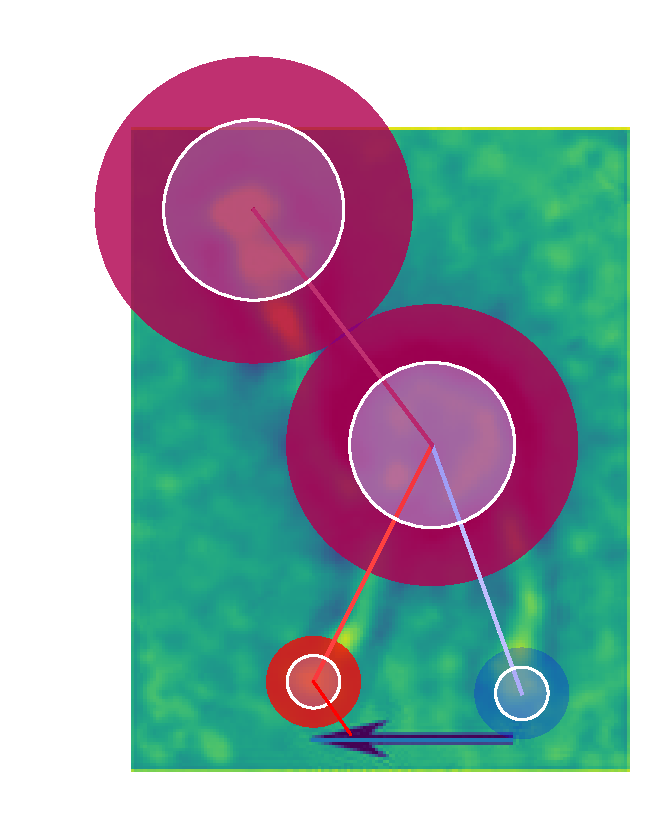
\includegraphics[width=0.3\columnwidth]{../../plots/burgess-model-figure.pdf}
	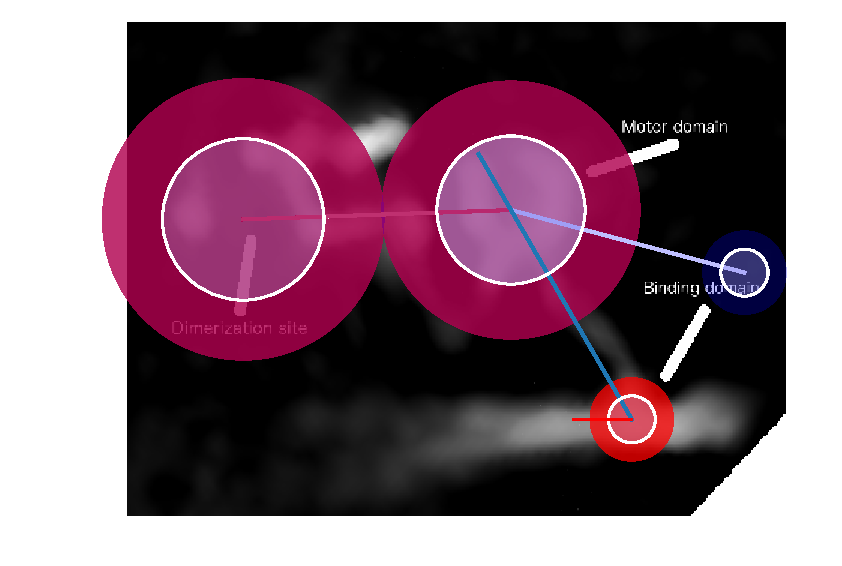
\includegraphics[width=0.5\columnwidth]{../../plots/grotjahn-model-figure.pdf}%
	\caption[Experimental Pictures of Dynein for Model Parameters]{\textbf{Experimental Pictures of Dynein for Model Parameters} \textit{Left:} Micrograph of both bound dynein with model domains to identify post-stroke equilbrium angles \cite{burgess2003dynein}.  \textit{Right:} Cryo-electron tomograph of one bound dynein for pre-stroke equilbrium angles \cite{grotjahn}.} 
	\label{fig:ParamsPics}
\end{figure}

However, these pictures do not help identify the binding rates ($k_b$, $k_{ub}$) and spring constants ($c_b$, $c_m$, $c_t$), thus making these parameters \textit{free variables} in the model. Fortunately, the Monte Carlo simulation can quickly optimize these free variables and fit different combinations of parameters to  different sets of experimental data. Since we want to replicate Yildiz's observations from Figure (\ref{fig:YildizCorrelation}), the free variables will be optimized according to the slope and y-intercept of the correlation. 

\subsection{Rate Constants}
\textit{Fitting our rate constants were a huge part of our model and how we made sure our dynein can match experimentalist results. Maybe bring up sticky rate???}

\section{Model Validation}
\textit{Any tests of our model to make sure the code is reasonably sound and that the physics makes sense. Make sure there is no bugs in code. What was the bug testing procedure.}

\section{Data Analysis} \label{sec:DataAna}
As mentioned earlier, the simulation can only collect statistics for a given initial binding domain distance, $L$. This limits the probability data of landing at a final position to be a function of $L$. However, the unsigned distance is insignificant when calculating the step length of either a trailing or leading step. This promotes the new naming scheme of using initial displacement, $x_i$, and final displacement $x_f$, when identifying the distance between the binding domains before and after the step. The displacement is the $x$ position of the unbounded binding domain during the step, where the origin is defined at the bounded binding domain. This implies a negative initial displacement for a trailing step and a positive initial displacement for a leading step. 

However, we still suffer with the simulation outputting a probability distribution of final displacements as a function of initial displacements. To properly reproduce Yildiz's stepping plot, we need a joint probability distribution with both $x_i$ and $x_f$ as variables. Using probability notation, we want $p(x_i,x_f)$ (the probability of $x_i$ \textit{and} $x_f$) but we have $p(x_f|x_i)$ (the probability of $x_f$ \textit{given} $x_i$). To solve this problem, we can use conditional probability and solve for $p(x_i,x_f)$, as shown below:


\[
	p(x_f|x_i)=\frac{p(x_i,x_f)}{p(x_i)},
\]
\begin{equation}
	p(x_i,x_f)=p(x_f|x_i)p(x_i).
\end{equation}
Now, we only need to find the probability density of initial displacements, $p(x_i)$. Since the initial displacement is simply a signed distance $L$, we can use the probability of unbinding for a trailing or leading step as a function of $L$ from Equation (\ref{eqn:ProbTrail}) to generate $p(x_i)$. In otherwords, Equation (\ref{eqn:ProbTrail}) gives us $p(x_i|L_i)$. We can relate the two by using Bayes' Theorem:

\begin{equation}
	p(x_i|L_i)=\frac{p(L_i|x_i)p(x_i)}{p(L_i)}.
\end{equation}
Since the probability of an initial distance given the initial displacement, $p(L_i|x_i)$, is always 1, we can simplify further,
\[
	p(x_i|L_i)=\frac{p(x_i)}{p(L_i)} 
\]

\begin{equation}
	p(x_i)=p(x_i|L_i)p(L_i).
\end{equation}
Now, the final step is to solve for the probability density of initial distance, $p(L_i)$. We can do so by solving a Detailed Balance Equation, where we define a transition matrix, $T=p(L_f|L_i)$. This equation will have the form,
\begin{equation}
	p(L_i)=T^np^0(L_i),
\end{equation}
where $T$ is raised to the $n$ number of steps to signify equilibrium for the probability of all distances $L$. $n$ is chosen to be arbitrarily large to ensure equilibrium after enough steps (??? FIXME this reasoning needs to be clearer. Ask Roundy.) To solve for $T$, we can use the previous probability distributions $p(x_f|x_i)$ and $p(x_i|L_i)$ to convert the probabilities to distances, as shown below:
\begin{align}
	T&=I(L_f|x_i)p(x_f|x_i)p(x_i|L_i)\\
	&=p(L_f|x_i)p(x_i|L_i)\\
	&=p(L_f|L_i),
\end{align}
where $I(L_f|x_i)$ is the identity matrix for converting $x_f$ into $L_f$. We have now solved for all the unknowns to generate a joint probability distribution of initial and final displacements, $p(x_i,x_f)$. 


